\section{Phương pháp}
\label{sec:phuongphap}

\subsection{Phân tích chất lượng dữ liệu}
Mục~\ref{sec:thieuchiso} đã nêu nhanh ba vấn đề; phần này phân tích sâu hai vấn đề chi phối thiết kế pipeline: cảm biến COD chết và đơn vị NH4.

\subsubsection{Cảm biến COD đã hỏng (bão hòa)}
COD diễn biến từ mức hợp lý $\sim$10 mg/L, trôi tăng dần rồi \emph{dính cứng} ở trần 558{,}8 mg/L (Hình~\ref{fig:cod}, Bảng~\ref{tab:cod}).

\begin{table}[h]
\centering\small
\caption{Diễn biến COD theo ngày (median) --- cảm biến trôi rồi chết.}
\label{tab:cod}
\begin{tabular}{lcc}
\toprule
\textbf{Giai đoạn} & \textbf{COD median (mg/L)} & \textbf{\% bản ghi $=558{,}8$} \\
\midrule
29/05 -- 05/06 & $\sim$10 & 0\% \\
06/06 -- 09/06 & 28 $\to$ 128 $\to$ 330 $\to$ 452 & 0\% \\
10/06 & 551 & 46\% \\
11/06 -- 20/06 & 558{,}8 & \textbf{100\%} \\
\bottomrule
\end{tabular}
\end{table}

\begin{figure}[h]
\centering
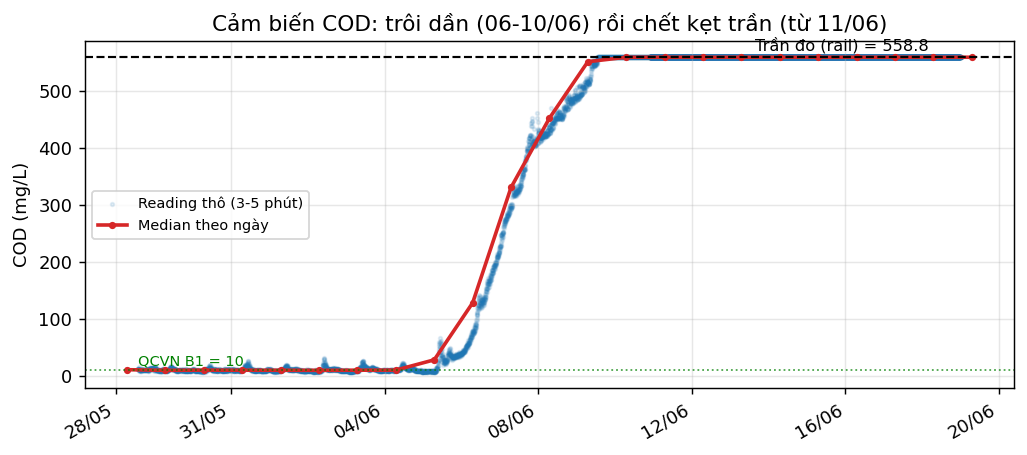
\includegraphics[width=\linewidth]{../figures/cod_timeline.png}
\caption{COD theo thời gian. Phẳng $\sim$10 mg/L tới 05/06, tăng vọt dạng chữ S (06--10/06), rồi kẹt cứng ở trần 558{,}8 --- dấu hiệu rõ của bão hòa cảm biến, không phải ô nhiễm thật.}
\label{fig:cod}
\end{figure}

\warnbox{\textbf{Kết luận:} 558{,}8 lặp lại y hệt trên 12.030 bản ghi liên tiếp (77{,}7\%), phương sai bằng 0 --- đặc trưng \textbf{bão hòa trần đo} (max-range rail), không phải ô nhiễm. Nhiều khả năng do bám bẩn/màng sinh học. Cần báo vận hành vệ sinh, hiệu chuẩn lại đầu dò.}

\subsubsection{Đơn vị NH4 chưa xác định}
NH4 thô dao động 77--160. Nếu là mg/L thì vô lý cho nước nuôi trồng; khả năng cao là $\mu$g/L ($\div 1000 \to 0{,}077$--$0{,}16$ mg/L, sát ngưỡng QCVN 0{,}1) hoặc tín hiệu thô. Ngoài ra cảm biến đo \textbf{NH4$^+$} (ít độc) trong khi QCVN đánh giá theo \textbf{NH3} (rất độc) --- không được ánh xạ thẳng.

\subsection{Kiến trúc 8 module}
\begin{center}\small
\texttt{fetch} $\to$ \texttt{quality} $\to$ \texttt{chemistry} $\to$
\texttt{monitor} $\to$ \texttt{impute} $\to$ \texttt{classify} $\to$ \texttt{report}
\end{center}

\begin{longtable}{ll}
\toprule
\textbf{Module} & \textbf{Trách nhiệm} \\
\midrule \endhead
\texttt{config.py}    & env, registry trạm, ngưỡng QCVN, dải QC, \texttt{NH4\_UNIT\_SCALE} \\
\texttt{chemistry.py} & Quy đổi NH4$^+\to$NH3 (Emerson) \\
\texttt{quality.py}   & QC cảm biến: lọc out-of-range + phát hiện rail/flatline \\
\texttt{fetch.py}     & MongoDB hoặc CSV $\to$ DataFrame; gộp ngày theo median \\
\texttt{monitor.py}   & Kiểm ngưỡng QCVN 10:2023 cột B1 \\
\texttt{impute.py}    & Nội suy thích nghi (dual-model 5/4 feature) + fallback median \\
\texttt{classify.py}  & Ghép đủ chỉ số $\to$ gọi \texttt{src.classification} \\
\texttt{report.py}    & CLI: in giám sát + phân loại + xuất xứ chỉ số \\
\bottomrule
\end{longtable}

\subsection{Quy đổi NH4 $\to$ NH3 (Emerson, 1975)}
\begin{equation}
f = \frac{1}{1 + 10^{(pK_a - pH)}}, \quad
pK_a = 0{,}09018 + \frac{2729{,}92}{T(\text{K})}, \quad
\text{NH3} = \text{NH4}_{\text{raw}} \cdot s \cdot f
\end{equation}
với $s$ là hệ số đơn vị (\texttt{NH4\_UNIT\_SCALE}, mặc định $0{,}001$). Ví dụ NH4$_{\text{raw}}=114{,}59$, pH$=7{,}95$, $T=30^\circ$C: $f\approx0{,}067 \Rightarrow$ NH3 $\approx 0{,}0077$ mg/L.

\warnbox{Đơn vị quyết định kết luận: $s=0{,}001$ cho NH3$=0{,}0077$ (\textbf{đạt}); $s=1{,}0$ cho NH3$=7{,}66$ (\textbf{vượt 76 lần}). Vì vậy đơn vị được tham số hóa và báo cáo luôn in rõ giả định.}

\subsection{Kiểm soát chất lượng (QC)}
Trước khi nội suy, QC chạy hai mức:
\begin{itemize}[nosep]
  \item \textbf{Lọc dòng} ngoài dải vật lý hợp lý (vd COD $\in(0,100)$ $\Rightarrow$ loại bỏ mọi reading $=558{,}8$).
  \item \textbf{Đánh giá chuỗi ngày}: chuỗi phẳng/kẹt trần (flatline, rail-stuck, $CV<10^{-3}$) $\to$ gắn nhãn \texttt{INVALID}.
\end{itemize}
Kết quả QC quyết định \emph{luồng xử lý} ở bước nội suy sau.

\subsection{Mô hình nội suy (XGBoost + LOO-CV theo trạm)}
\label{sec:model}
Ý tưởng: học từ \emph{dữ liệu quan trắc thật} mối quan hệ giữa các chỉ số mà sensor đo được và các chỉ số còn thiếu, rồi áp lên dữ liệu sensor realtime (Hình~\ref{fig:method}).

\begin{figure}[h]
\centering
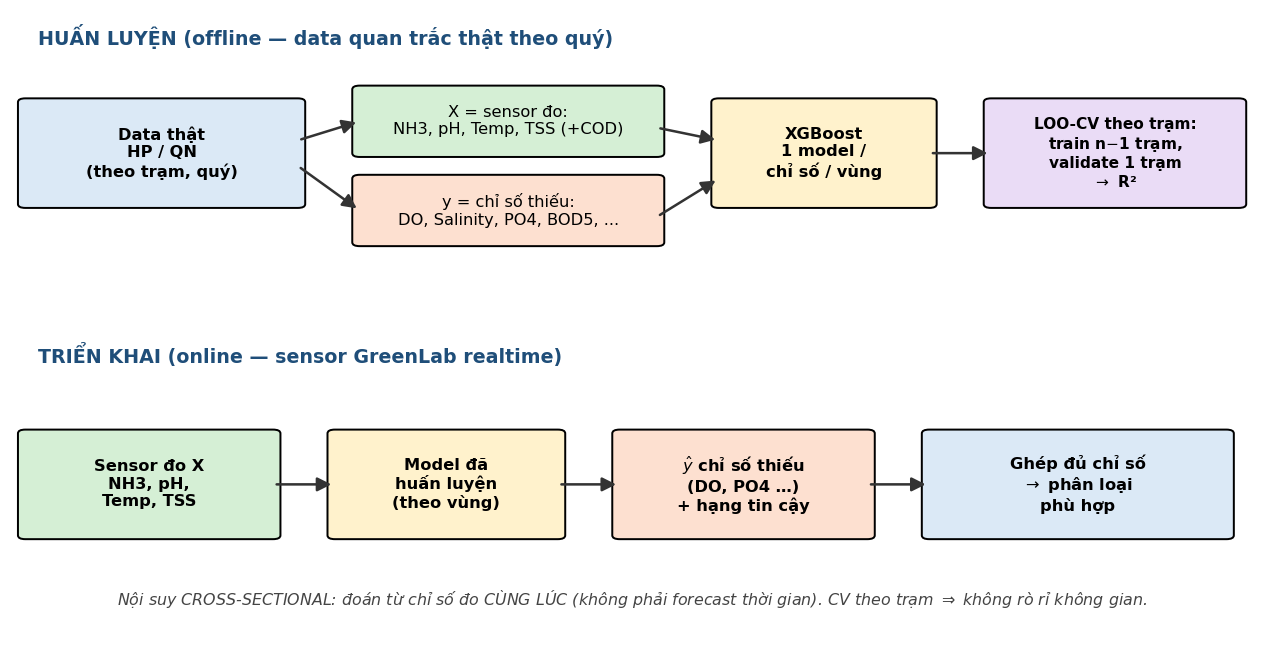
\includegraphics[width=\linewidth]{../figures/impute_method.png}
\caption{Phương pháp nội suy. \textbf{Huấn luyện} (offline): từ data quý HP/QN, đầu vào $X$ = chỉ số sensor đo được, đầu ra $y$ = chỉ số thiếu; mỗi chỉ số một XGBoost; kiểm định LOO-CV theo trạm. \textbf{Triển khai} (online): sensor đo $X$ $\to$ model $\to$ $\hat{y}$ $\to$ phân loại.}
\label{fig:method}
\end{figure}

\begin{itemize}[nosep]
  \item \textbf{Đầu vào} $X$ = chỉ số sensor có: \texttt{[NH3, pH, Temperature, TSS]} ($+$ \texttt{COD} khi sống). Mô phỏng đúng bộ chỉ số GreenLab cấp.
  \item \textbf{Đầu ra} $y$ = chỉ số thiếu cần đoán: DO, \textbf{Salinity}, PO4, BOD5, Transparency, Alkalinity. \emph{Một} mô hình cho \emph{mỗi} chỉ số $\times$ \emph{mỗi} vùng.
  \item \textbf{Kiểm định} = \textbf{Leave-One-Station-Out CV}: huấn luyện trên $n-1$ trạm, dự đoán trạm bị giữ lại, lặp cho mọi trạm rồi gộp $\to R^2$. Chia theo \emph{trạm} (không theo thời gian) để tránh rò rỉ không gian.
\end{itemize}

\warnbox{Đây là nội suy \textbf{cross-sectional} --- đoán giá trị một chỉ số từ các chỉ số đo \emph{cùng thời điểm}, \emph{không phải} dự báo (forecast) theo thời gian. Vì vậy chỉ cần một bản ghi sensor là suy ra được, không cần chuỗi lịch sử.}

\subsubsection{Thuật toán: XGBoost (gradient boosting trees)}
Mỗi mô hình nội suy là một \textbf{XGBoost} (\texttt{XGBRegressor}) --- gradient boosting trên cây quyết định. Lý do chọn:
\begin{itemize}[nosep]
  \item \textbf{Phù hợp dữ liệu bảng}, ít mẫu (HP chỉ 216 dòng): cây boosting học tốt quan hệ phi tuyến mà không cần chuẩn hóa đặc trưng, ít nhạy outlier hơn mô hình tuyến tính.
  \item \textbf{Tương quan phi tuyến} giữa chỉ số sinh-hóa (vd Salinity vs NH3/TSS theo gradient cửa sông) — cây nắm được, hồi quy tuyến tính thì không.
  \item \textbf{Nhất quán với hệ thống chính} của đồ án (XGBoost đã là phương pháp lõi cho dự báo + phân loại), dễ tái dùng hạ tầng.
\end{itemize}

\begin{table}[h]
\centering\small
\caption{Siêu tham số XGBoost (đồng nhất mọi chỉ số/vùng).}
\label{tab:xgb}
\begin{tabular}{ll}
\toprule
\textbf{Tham số} & \textbf{Giá trị} \\
\midrule
\texttt{n\_estimators} & 100 (số cây) \\
\texttt{max\_depth}    & 4 (giữ cây nông, chống overfit data nhỏ) \\
\texttt{learning\_rate}& 0{,}1 \\
\texttt{random\_state} & 42 (tái lập) \\
objective & \texttt{reg:squarederror} (hồi quy) \\
\bottomrule
\end{tabular}
\end{table}

Số cây vừa phải $+$ cây nông là lựa chọn có chủ đích cho tập huấn luyện nhỏ: đủ học quan hệ chính nhưng tránh khớp quá. Kết quả LOO-CV (Mục~\ref{sec:r2}) cho thấy mô hình \emph{không} tự khớp ảo --- phần lớn chỉ số R² thấp/âm đúng như kỳ vọng khi không có tín hiệu.

\subsection{Hai luồng xử lý của bước nội suy}
\label{sec:hailuong}
Phần suy ra chỉ số thiếu được tổ chức theo \textbf{hai trục quyết định độc lập}. Trục nào cũng do dữ liệu thực ép ra, không phải lựa chọn tùy ý.

\subsubsection{Luồng 1 --- thích nghi theo trạng thái COD (5-feature vs 4-feature)}
Vì cảm biến COD chết phần lớn thời gian, mô hình nội suy phải \emph{thích nghi} theo kết quả QC của COD:
\begin{itemize}[nosep]
  \item \textbf{COD VALID} (giai đoạn đầu, $<6$\% reading): dùng bộ \textbf{5-feature} [COD, NH3, pH, Temp, TSS]. Các dòng COD lỗi đã bị QC \emph{cắt bỏ} khỏi tập huấn luyện/suy luận.
  \item \textbf{COD INVALID} (đa số): rớt COD, dùng bộ \textbf{4-feature} [NH3, pH, Temp, TSS]. Không bịa COD bằng median (sẽ kéo lệch toàn bộ).
\end{itemize}
Hai bộ được huấn luyện sẵn; QC chọn bộ tại thời điểm chạy. Ngày 20/06 (COD chết) $\to$ tự động dùng 4-feature.

\subsubsection{Luồng 2 --- huấn luyện theo vùng (HP-only vs HP+QN gộp)}
Mô hình nội suy được train trên \emph{dữ liệu quan trắc thật} theo quý. Câu hỏi: trạm Cát Bà (HP) nên học từ data nào?
\begin{itemize}[nosep]
  \item \textbf{HP-only} (216 dòng, 14 trạm Hải Phòng) --- cùng vùng với trạm đích.
  \item \textbf{HP+QN gộp} (thêm 1.552 dòng, 97 trạm Quảng Ninh) --- nhiều mẫu hơn nhưng khác chế độ thủy văn.
\end{itemize}
Hai vịnh khác chế độ làm quan hệ sensor$\to$DO mâu thuẫn khi gộp; kết quả (Mục~\ref{sec:r2}) cho thấy tách HP-only \emph{cứu} được dự đoán DO mà gộp đã phá. Vì vậy chọn huấn luyện \textbf{riêng theo vùng}.

\subsubsection{Kết hợp hai luồng}
Bảng~\ref{tab:hailuong} là ma trận $2\times2$. Mỗi ô là một bộ mô hình riêng; thực thi chọn ô theo (vùng trạm $\times$ trạng thái COD).

\begin{table}[h]
\centering\small
\caption{Ma trận hai luồng. Trạm Cát Bà 20/06 rơi vào ô \textbf{HP-only $\times$ 4-feature}.}
\label{tab:hailuong}
\begin{tabular}{lcc}
\toprule
& \textbf{COD VALID (5-feat)} & \textbf{COD INVALID (4-feat)} \\
\midrule
\textbf{HP-only}     & 5 cột$^*$ & 4 cột \textbf{(Cát Bà 20/06)} \\
\textbf{HP+QN gộp}   & 5 cột & 4 cột \\
\bottomrule
\end{tabular}

{\footnotesize $^*$ Data HP không có cột COD/BOD5/Alkalinity nên ``5-feature'' ở HP thực chất chỉ 4 cột; code lưu đúng danh sách cột mỗi vùng (\texttt{feat\_cols.json}) để vector suy luận không lệch.}
\end{table}

Sau khi nội suy, kiểm định \textbf{LOO-CV theo trạm} và phân hạng theo \textbf{chính sách 3 mức tin cậy} (chi tiết Mục~\ref{sec:r2}): $R^2\ge0{,}4$ dùng model (ML-mạnh); $0{,}2\le R^2<0{,}4$ vẫn dùng nhưng gắn cờ độ tin thấp (ML-yếu); $R^2<0{,}2$ thay bằng trung vị vùng. Hai chỉ số artifact (BOD5, Alkalinity) bị loại bất kể $R^2$. Cuối cùng ghép \texttt{measured} $\oplus$ \texttt{imputed} $\oplus$ \texttt{defaulted} $\to$ chấm điểm piecewise-linear theo breakpoint chuyên gia (\texttt{src.classification}).
